\documentclass{beamer}
\usepackage{amsopn}

\DeclareMathOperator{\conv}{conv}
\DeclareMathOperator{\average}{average}
\DeclareMathOperator{\support}{support}
\DeclareMathOperator{\boundary}{\partial}

\usepackage{beamerthemesplit}
 
%\usepackage{amsthm}

\newcommand{\centeripe}[1]{\begin{center}\Ipe{#1}\end{center}}
\newcommand{\comment}[1]{}

\newcommand{\centerpsfig}[1]{\centerline{\psfig{#1}}}

\newcommand{\seclabel}[1]{\label{sec:#1}}
\newcommand{\Secref}[1]{Section~\ref{sec:#1}}
\newcommand{\secref}[1]{\mbox{Section~\ref{sec:#1}}}

\newcommand{\alglabel}[1]{\label{alg:#1}}
\newcommand{\Algref}[1]{Algorithm~\ref{alg:#1}}
\newcommand{\algref}[1]{\mbox{Algorithm~\ref{alg:#1}}}

\newcommand{\applabel}[1]{\label{app:#1}}
\newcommand{\Appref}[1]{Appendix~\ref{app:#1}}
\newcommand{\appref}[1]{\mbox{Appendix~\ref{app:#1}}}

\newcommand{\tablabel}[1]{\label{tab:#1}}
\newcommand{\Tabref}[1]{Table~\ref{tab:#1}}
\newcommand{\tabref}[1]{Table~\ref{tab:#1}}

\newcommand{\figlabel}[1]{\label{fig:#1}}
\newcommand{\Figref}[1]{Figure~\ref{fig:#1}}
\newcommand{\figref}[1]{\mbox{Figure~\ref{fig:#1}}}

\newcommand{\eqlabel}[1]{\label{eq:#1}}
\newcommand{\eqref}[1]{(\ref{eq:#1})}

\newtheorem{thm}{Theorem}{\bfseries}{\itshape}
\newcommand{\thmlabel}[1]{\label{thm:#1}}
\newcommand{\thmref}[1]{Theorem~\ref{thm:#1}}

\newtheorem{lem}{Lemma}{\bfseries}{\itshape}
\newcommand{\lemlabel}[1]{\label{lem:#1}}
\newcommand{\lemref}[1]{Lemma~\ref{lem:#1}}

\newtheorem{cor}{Corollary}{\bfseries}{\itshape}
\newcommand{\corlabel}[1]{\label{cor:#1}}
\newcommand{\corref}[1]{Corollary~\ref{cor:#1}}

\newtheorem{obs}{Observation}{\bfseries}{\itshape}
\newcommand{\obslabel}[1]{\label{obs:#1}}
\newcommand{\obsref}[1]{Observation~\ref{obs:#1}}

\newtheorem{assumption}{Assumption}{\bfseries}{\rm}
\newenvironment{ass}{\begin{assumption}\rm}{\end{assumption}}
\newcommand{\asslabel}[1]{\label{ass:#1}}
\newcommand{\assref}[1]{Assumption~\ref{ass:#1}}

\newcommand{\proclabel}[1]{\label{alg:#1}}
\newcommand{\procref}[1]{Procedure~\ref{alg:#1}}

\newtheorem{rem}{Remark}
\newtheorem{op}{Open Problem}

\newcommand{\etal}{\emph{et al}}

\newcommand{\voronoi}{Vorono\u\i}
\newcommand{\ceil}[1]{\left\lceil #1 \right\rceil}
\newcommand{\floor}[1]{\left\lfloor #1 \right\rfloor}



\newcommand{\pin}{p_{\mathsf{in}}}
\newcommand{\pout}{p_{\mathsf{out}}}
\DeclareMathOperator{\cost}{cost}
\DeclareMathOperator{\depth}{depth}

\title{Distribution-Sensitive Point Location\\ in Convex Subdivisions}
\author{Pat Morin}
\institute{Carleton University}
\date{December 6, 2006 \\ McGill University}

\begin{document}

\frame{\titlepage}

\section[Outline]{}
\frame{\tableofcontents}

\section{Introduction}
\subsection{Planar Point Location}
\frame
{
  \frametitle{Planar Point Location}
  \begin{itemize}
  \item Preprocess a planar subdivision $G$ so that, for any query
point $p\in\R^2$, the we can quickly determine the face of $G$
that contains $p$
  \begin{center}
  \only<1>{\includegraphics{pl-1}}
  \only<2>{\includegraphics{pl-2}}
  \only<3>{\includegraphics{pl-3}}
  \end{center}
  \end{itemize}
}

\subsection{History}

\frame
{
  \frametitle{The 1980s}
  \begin{itemize}
  \item<1-> After a few initial attempts, optimal $O(n)$ space, $O(\log
n)$ query time solutions were obtained by
  \begin{itemize}
   \item<2-> Kirkpatrick (1983) --- Independent set removal
   \item<3-> Edelsbrunner, Guibas, and Stolfi (1986) --- Fractional cascading
   \item<4-> Sarnak and Tarjan (1986) --- Persistence
   \item<5-> Mulmuley (1990) --- Randomized incremental construction
  \end{itemize}
  \end{itemize}
}

\frame
{
  \frametitle{The 1990s}
  \begin{itemize}
  \item<1-> Then we started carefully studying the constants:
   \item<2-> Goodrich, Orletsky, and Ramaiyer (1997)
   \begin{itemize}
      \item<3-> $O(n)$ space, $2\log n + o(\log n)$ standard comparisons
      \item<4-> Conjectured that $2\log n$ is optimal for linear space structures
   \end{itemize}
   \item<5-> Adamy and Seidel (1998)
   \begin{itemize}
      \item<6-> $O(n)$ space, $\log n + \sqrt{2}\log\log n +
o(\log\log n)$ standard comparisons
      \item<7-> Optimal up to the second term
   \end{itemize}
  \end{itemize}
}

\frame
{
  \frametitle{The New Millenium --- A New Era of Sensitivity}
  \begin{itemize}
  \item<1-> Adamy and Seidel's result closes the problem of the
	worst-case complexity of planar point location
  \item<2-> What about the average case?
  \item<3-> Assume the point $p$ is selected according to a
	probability measure $D$ over $\R^2$
  \item<4-> Given $(G,D)$ can we optimize the expected cost of
	locating $p$?
  \end{itemize}
}

\frame
{
  \frametitle{Defining Optimality}
  \begin{itemize}
   \item<1-> We need a way of knowing when a point location structure
	is optimal
   \item<2-> $D$ induces a distribution over the faces of $G$
   \item<3-> Let $p_i=\Pr\{\mbox{$p$ is contained in face $i$}\}$
   \item<4-> \textbf{Theorem (Shannon 1948):}
     For any data structure $X$ that makes only binary decisions, the
expected number of decisions is at least
   \[
      \mu_D(X) \ge H(p_1,\ldots,p_f) = \sum_{i=1}^f p_i\log(1/p_i)  \enspace .
   \]
  \end{itemize}
}

\frame
{
   \frametitle{Distribution-Sensitive Point Location: Results}
   \begin{itemize}
   \item<1-> Arya, Cheng, Mount, and Ramesh (2000)
    \begin{itemize}
      \item<1->For convex subdivisions: $O(n^2)$ space, $2H+o(H)$ comparisons
      \item<1->For convex subdivisions: $O(n)$ space, $4H+o(H)$ comparisons
      \item<1->Requires that $x$ and $y$ coordinates of $p$ are independent
    \end{itemize}
   \item<2-> Arya, Malamatos, and Mount (2000)
    \begin{itemize}
      \item<2->For triangulations: $O(n\log n)$ space, $H+o(H)$ comparisons
    \end{itemize} 
    \item<3-> Arya, Malamatos, and Mount (2001a)
    \begin{itemize}
      \item<3->For triangulations: $O(n\log^* n)$ space, $H+o(H)$ comparisons
    \end{itemize} 
    \item<4-> Arya, Malamatos, and Mount (2001b)
    \begin{itemize}
      \item<4->For triangulations: $O(n)$ space, $O(H)$ comparisons (randomized)
    \end{itemize} 
    \item<5-> Iacono (2001)
    \begin{itemize}
      \item<5->For triangulations: $O(n)$ space, $O(H)$ comparisons (deterministic)
    \end{itemize} 
   \end{itemize}


}

\section{Point-in-Polygon Testing}
\frame
{
   \frametitle{Point-in-Polygon Testing}
   \begin{itemize}
   \item<1-> It looks like distribution-sensitive point location is 
	well understood, but\ldots
   \item<2-> A simple question: $P$ is a convex $n$-gon, $D$ is a
	probability measure over $\R^2$
   \item<3-> Preprocess $(P,D)$ so that we can quickly determine if a
point $p$, distributed according to $D$ is inside or outside $P$
   \item<4-> None of the above results apply
   \end{itemize}
}

\frame
{
   \frametitle{Difficulties I}
   \begin{itemize}
   \item<1-> We will want to prove that our data structure is optimal
   \item<2-> But there are only two outcomes, so
     \[ H= \pin\log (1/\pin) + \pout\log(1/\pout) \le 1  \]
   \item<3-> We can't always match the entropy lower bound!
   \end{itemize}
}

\frame
{
   \frametitle{Difficulties}
   \begin{itemize}
     \item<1-> We could try to triangulate $P$ and apply a result for 
	triangulations\\
     \only<1>{\centerline{\includegraphics[scale=.6]{problema-1}}
        -}       
     \only<2>{\centerline{\includegraphics[scale=.6]{problema-2}}
        $H= \sum_{i=1}^f (c/f)\log (f/c) = \Theta(\log f)$ }       
     \only<3->{\centerline{\includegraphics[scale=.6]{problema-3}}
        $H= p_1\sum_{i=1}^3 p_i\log(1/p_i) = O(1)$ }       
     \item<4-> Choosing correct triangulation is critical
   \end{itemize}
}

\frame
{
   \frametitle{The Data Structure}
   \begin{itemize}
    \item<1-> We define a binary \emph{triangle tree} $T=T(P,D)$
    \item<2-> The vertices of $T$ correspond to triangles
    \item<3-> Each triangle approximates a section of the boundary of $P$
    {\includegraphics{ssplit-a}}
    \only<4>{\includegraphics{ssplit-b}}%
    \only<5>{\includegraphics{ssplit-c}}%
    \only<6>{\includegraphics{ssplit-d}}%
    \only<7->{\includegraphics{ssplit-e}}%
    \item<4-> Each internal node is split into two triangles
    \item<8-> The leaves of $T$ correspond to triangles completely
	contained in $P$
   \end{itemize}
}

\frame
{
   \frametitle{The Triangle Tree (Example)}
   \includegraphics{tree}
   Each level of $T$ is an approxmation of $\partial P$
}


\frame
{
   \frametitle{Searching in $T$}
   \begin{itemize}
     \item<1-> Searching in $T$ is done top-down, starting at the root
     \item<2-> For each triangle either:
      \begin{itemize}
        \item<3-> We finish the search:\\
          \includegraphics{finish}
        \item<4-> We recurse on one of the two children:\\
          \includegraphics{recurse}
      \end{itemize}
   \end{itemize}
}

\frame
{
   \frametitle{Analysis of the Triangle Tree}
   \begin{itemize}
   \item<1-> Let $\Pr(v)$ denote the probability that a search for $p$ 
	finishes at node $v\in T$
   \item<2-> Note that, if $v$ is at depth $i$ in $T$ then $\Pr(v)\le 1/2^i$
   \item<3-> So, the expected cost of searching in $T$ is at most
   \begin{eqnarray*}
      \mu_D(T) 
    &=& O(1) + O(1)\times\sum_{v\in T} \Pr(v)\times\depth(v) \\
       &\le& O(1)+O(1)\times \sum_{v\in T} \Pr(v)\log(1/\Pr(v))
   \end{eqnarray*}
   \end{itemize}

}

\frame
{
	\frametitle{Review and Lookahead}
	\begin{itemize}
	\item<1-> We have a triangle tree $T$ whose search time is
	 \[ \mu_D(T) \le O(1)+O(1)\times \sum_{v\in T} \Pr(v)\log(1/\Pr(v))
         \]
	and we want to show that this is optimal 
        \item<2-> We will show that every point location structure $X$ for
	$P$ is also a point location structure for the triangles of
$T$, so Shannon's Theorem gives
	 \[ \mu_D(X) \ge \sum_{v\in T} \Pr(v)\log(1/\Pr(v))
         \]
        \item<3-> Well, not exactly\ldots
          \begin{itemize}
		\item<4-> $X$ can distinguish between most (but not all) triangles of $T$
		\item<5-> But this will be good enough
          \end{itemize}
	\end{itemize}
}

\frame
{
   \frametitle{Linear Decision Trees}
   \begin{itemize}
     \item<1-> We need to fix a model of computation for the lower bound
     \item<2-> A \emph{linear decision tree} is a binary where
       \begin{itemize}
          \item Each internal node is labelled with a linear inequality
          \item Each leaf is labelled with \emph{in} or \emph{out}
          \item For every $p\in\R^2$ the search path for $p$ finishes at 
           a leaf labelled \emph{in} if and only if $p\in P$
       \end{itemize}
     \item<3-> Every point location structure in the
	introduction can be expressed as a linear decision tree
   \end{itemize}
}

\frame
{
	\frametitle{Linear Decision Tree Example}
        \only<1>{\includegraphics{ld-a}}%
        \only<2>{\includegraphics{ld-b}}%
        \only<3>{\includegraphics{ld-c}}%
        \only<4>{\includegraphics{ld-d}}%
        \only<5>{\includegraphics{ld-e}}%
        \only<6>{\includegraphics{ld-e}}%
}


\frame
{
	\frametitle{A Non-Trivial Lower Bound}
        \begin{itemize}
          \item<1-> Suppose we have this polygon $P$ and this distribution $D$:
            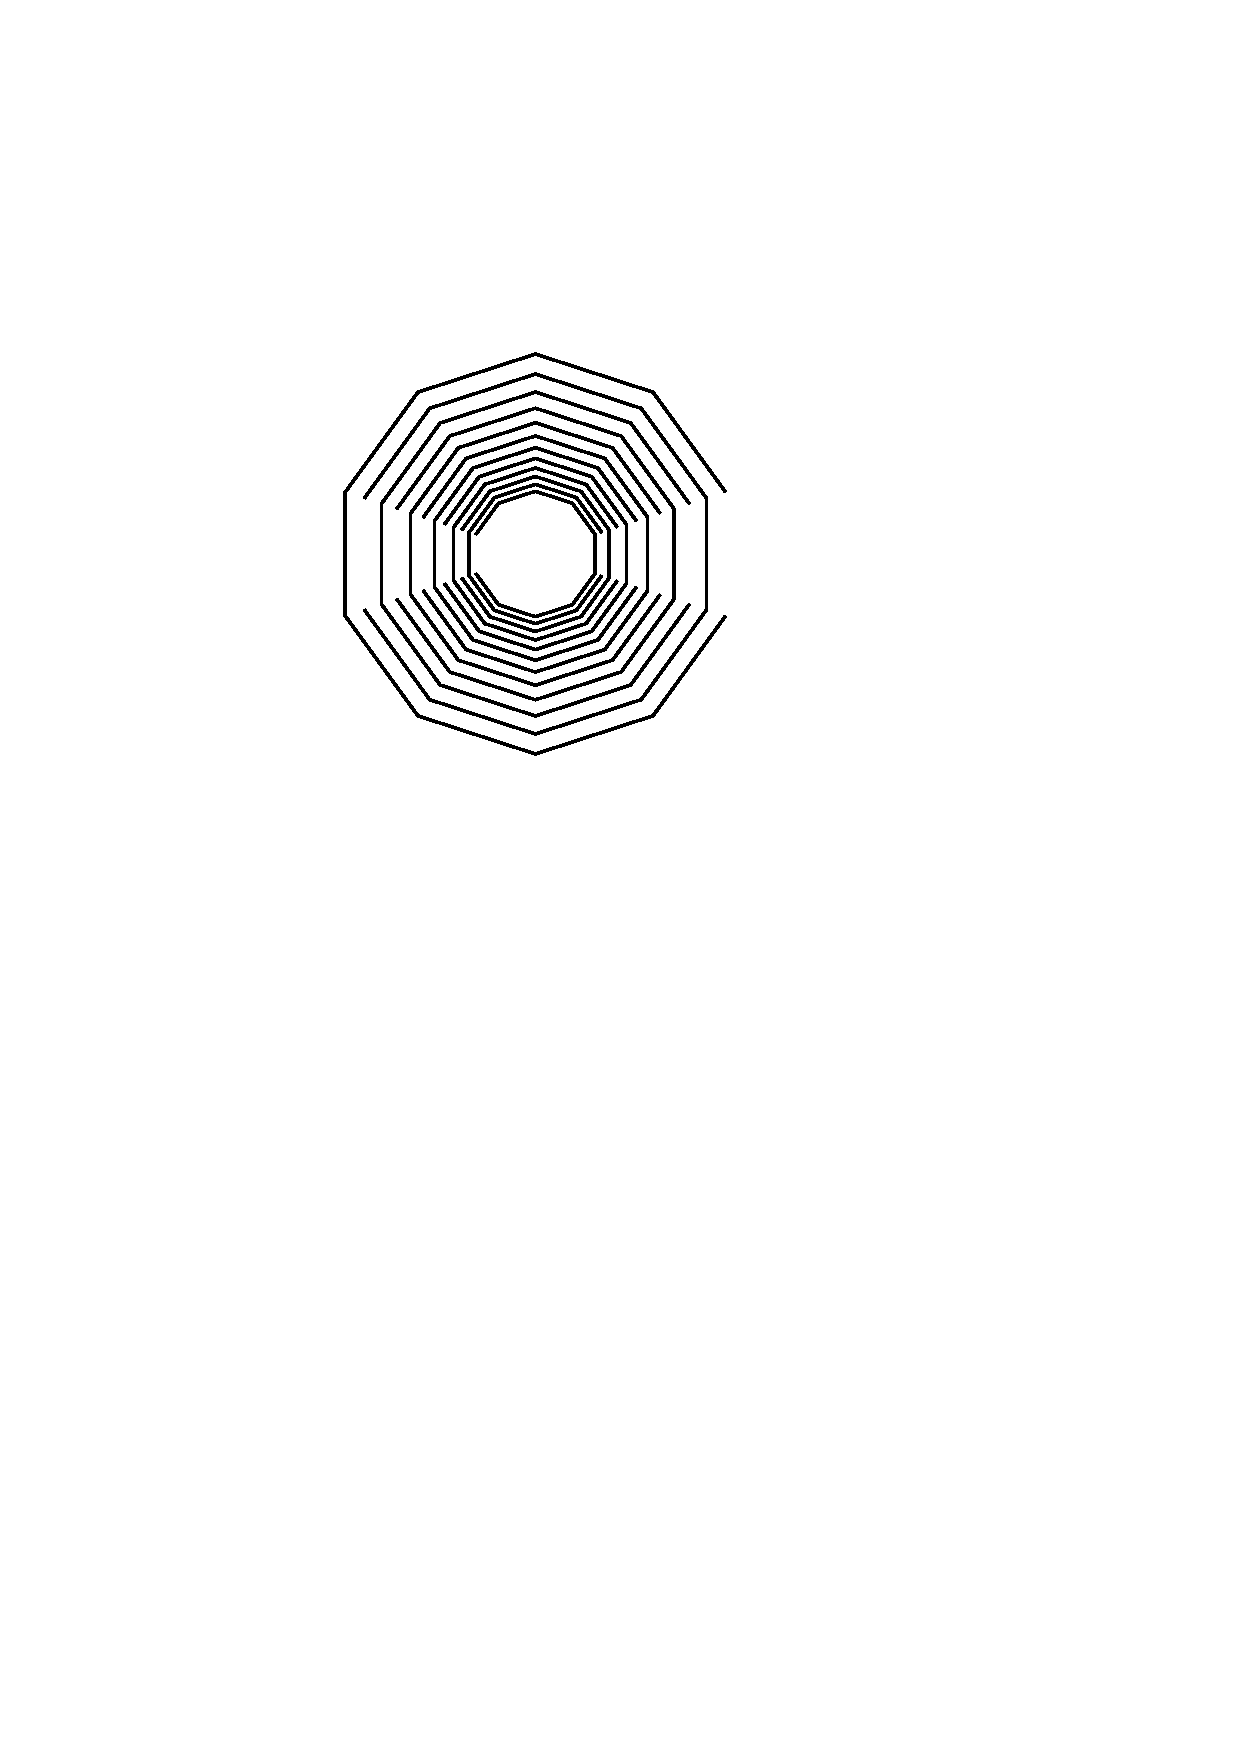
\includegraphics{lower-bound}
          \item<2-> \textbf{Lemma 0:} Any linear decision tree $X$ for
testing if $p\in P$ has 
\[  \mu_D(X)\ge \frac{1}{2}\sum_{i=1}^{11} p_i\log(1/p_i)  \]
        \end{itemize} 
}


\frame
{
	\frametitle{Proof of Lemma 0}
        \begin{itemize}
           \item<1->We first prove a lower bound for the \emph{chord tree} model\\
            \only<1>{\includegraphics{lb-proof-a}}%
            \only<2>{\includegraphics{lb-proof-b}}%
            \only<3>{\includegraphics{lb-proof-c}}%
            \only<4->{\includegraphics{lb-proof-d}}%
           \item<2->Let $C_1,\ldots,C_{11}$ be the components of 
               $\support(D)\setminus \boundary P$

           \item<3->For any $p\in C_i$ and $q\in C_j$ $i\neq j$, $p$ and $q$
               must live in different leaves of the chord tree

           \item<4->By labelling leaves of the chord tree $T_C$
		appropriately we obtain a
               point location structure for $C_1,\ldots,C_{11}$ \\
           $\Rightarrow$ By Shannon's Theorem $\mu_D(T_C) \ge \sum_{i=1}^{11}p_i\log (1/p_i)$
           \item<5->Any line intersects $\support(D)$ in at most 2 chords
		\hfill{\qed}
        \end{itemize}
}


\frame
{
    \frametitle{Using Lemma 0}
    \begin{itemize}
	\item<1-> Let $V\subseteq V(T)$ be such that no vertex in
$V$ is an ancestor of any other vertex in $V$
        \item<2-> The triangles of $V$ look like this:\\
	\includegraphics{using-lemma0}
        \item<3->Let $D_V$ be the measure $D$ conditioned on the
search completing at a node in $V$
        \item<4->\textbf{Lemma 1:} For any linear decision tree $X$
        \[ \mu_{D_V}(X) \ge \frac{1}{4}\sum_{v\in V} \Pr(v\mid V)\log (1/\Pr(v\mid V))
         \]
    \end{itemize}
}

\frame{
     \frametitle{Review}

     \begin{itemize}
	\item<1-> We have a triangle tree $T$ whose search time is
	 \[ \mu_D(T) \le O(1)+O(1)\times \sum_{v\in T} \Pr(v)\log(1/\Pr(v))
         \]
        \item<2-> For any linear decision tree $X$ and any
	\emph{genetically independent set} $V\subseteq V(T)$ of
	 \[ \mu_{D_V}(X) \ge \sum_{v\in V} \Pr(v\mid V)\log(1/\Pr(v\mid V))
         \]
        \item<3-> For any partition of $V(T)$ into genetically
independent sets $V_1,\ldots,V_k$, and any linear decision tree $X$,
	 \[ \mu_D(X) \ge \frac{1}{4}\sum_{i=1}^k\Pr(V_i)\sum_{v\in V_i} \Pr(v\mid
V_i)\log(1/\Pr(v\mid V_i))
         \]
     \end{itemize}
}


\frame
{
	\frametitle{Review (Cont'd)}

 	\begin{itemize}
	\item<1-> We're now dangerously close to matching upper and lower bounds
        \begin{eqnarray*}
	\mu_D(X) &\ge &\frac{1}{4}\sum_{i=1}^k
	   \Pr(V_i)\sum_{v\in V_i} \Pr(v\mid V_i)\log(1/\Pr(v\mid V_i)) \\
	& = &\frac{1}{4}\sum_{i=1}^k\sum_{v\in V_i} 
		\Pr(v)\log(1/\Pr(v\mid V_i)) \\
	& = &\frac{1}{4}\sum_{i=1}^k\sum_{v\in V_i} 
		\Pr(v)(\log(1/\Pr(v))-\log(1/\Pr(V_i)))
	\end{eqnarray*}
	\item<2-> The trick is to pick our $V_i$s so that
$\log(1/\Pr(V_i))$ is small
	\end{itemize}

}


\frame
{
	\frametitle{Picking the $V_i$s}

	\begin{itemize}
	\item<1-> Let
	\[
		V_i=\{v\in V(T) :1/2^{i-1} \le \Pr(v) \le 1/2^i \}
	\]
	\item<2-> But these $V_i$ are not genetically independent!
 	\item<3-> While $|V_i|\ge 2^{\alpha i}$
	   \begin{itemize}
		\item $V_{i,j}$ is a genetically independent subset of
			$V_i$ with size $2^{\alpha i}/i$
		\item $V_i\gets V_i\setminus V_{i,j}$
		\item $j\gets j+1$
	   \end{itemize}
	\item<4-> With the right $\alpha$ and some work, we can show that
	\begin{eqnarray*}
	\mu_D(X) & \ge & \frac{1}{4}\sum_{i,j}\sum_{v\in V_{i,j}} 
		\Pr(v)(\log(1/\Pr(v))-\log(1/\Pr(V_{i,j}))) \\
	& \ge & \left(\frac{1}{4}-\epsilon\right)\sum_{v\in T}\Pr(V)\log(1/\Pr(V)) -
O(1)
	\end{eqnarray*}
	\end{itemize}
}



\comment{
    
\subsection{Zonoid Depth}
\frame
{
   \frametitle{Zonoid Depth}
   \begin{itemize}
   \item<1-> Recall the definition of the \emph{convex hull}
    \[ \conv(S) = \left\{\sum_{p\in S} p\lambda_p : 
         \mbox{$0\le\lambda_p\le 1$ and $\sum_{p\in S}\lambda_p = 1$} 
        \right\} 
    \]
   \item<2-> Change it slightly to get the \emph{$k$-zonoid}
    \[ Z_k(S) = \left\{\sum_{p\in S} p\lambda_p : 
         \mbox{$0\le\lambda_p\le 1/k$ and $\sum_{p\in S}\lambda_p = 1$} 
        \right\} 
    \]
   \item<3-> Note that $Z_1(S)=\conv(S)$ and $Z_n(S)=\{\average(S)\}$ 
   \item<4-> The \emph{zonoid depth} of $p$ is 
     \[ Z(p,S)=\max\{k : p\in Z_k(S)\} \]
   \end{itemize}
}

\frame
{
    \frametitle{Zonoid Depth}
     \only<1>{\centerline{\includegraphics{zonoid-eg-ps}} 
	$S$} 
     \only<2>{\centerline{\includegraphics{zonoid-eg-1}}
	$S,Z_1(S)$}
     \only<3>{\centerline{\includegraphics{zonoid-eg-2}}
	$S,Z_1(S),Z_2(S)$}
     \only<4>{\centerline{\includegraphics{zonoid-eg-3}}
	$S,Z_1(S),Z_2(S),Z_3(S)$}
     \only<5>{\centerline{\includegraphics{zonoid-eg-4}}
	$S,Z_1(S),Z_2(S),Z_3(S),Z_4(S)$}
     \only<6>{\centerline{\includegraphics{zonoid-eg-5}}
	$S,Z_1(S),Z_2(S),Z_3(S),Z_4(S),Z_5(S)$}
     \only<7>{\centerline{\includegraphics{zonoid-eg-6}}
	$S,Z_1(S),Z_2(S),Z_3(S),Z_4(S),Z_5(S),Z_6(S)$}
}

\frame
{
   \frametitle{Applications of (Zonoid) Depth}
   \begin{itemize}
    \item<1-> Exploratory data analysis (visualization)
    \item<2-> Multivariate statistics
    \item<3-> Clustering
    \item<4-> Outlier removal
    \item<5-> Machine learning (classification)
    \item<6-> Soft-margin support vector machines
   \end{itemize}
}


\subsection{Zonoid Depth Computation}
\frame
{
  \frametitle{Zonoid Depth Computation}
  \begin{itemize}
  \item<1-> Given $p$ and $S$ compute the zonoid depth of $p$
w.r.t. $S$
  \item<2-> A necessary subroutine for most applications
  \item<3-> Known algorithms:
     \begin{itemize}  
       \item<4-> Polynomial: Solve a linear program in $\lambda_p$ 
		variables ($n$ variables and $O(n)$ inequalities)
       \item<5-> Bern and Eppstein 2001:  $O(n(Ld\log n)^c)$ time where $L$
            is the bit precision of the input  (uses ellipsoid method)
       \item<6-> Gopala and Morin 2004: $O(n)$ expected time, but only
            for $d=2$
       \item<7-> Here: $O(n)$ expected time for any constant $d$ (but
            with a superpolynomial dependence on $d$)
     \end{itemize}
     \item<8-> In this talk we focus mainly on the \emph{decision 
          problem}:  \\ ``Is $p\in Z_k(S)$?''
  \end{itemize}
}


\section{The Algorithm}

\subsection{Finding a Zonoid Vertex}

\frame{
   \frametitle{Finding a Zonoid Vertex}
   To Find the extreme vertex of $Z_k(S)$ in direction $\overrightarrow{w}$:
   \only<1>{\includegraphics{project-1}}
   \only<2>{\includegraphics{project-2}}
   \only<3>{\includegraphics{project-3}}
   \only<4>{\includegraphics{project-4}}
   \begin{enumerate}
     \item<2->Project points of $S$ onto $\overrightarrow{w}$
     \item<3->In $O(n)$ time, find the largest $k$ points in the projection 
     \item<4->Take the average of these $k$ points ($\lambda_p=1/k$)
   \end{enumerate}
}

\frame
{
   \frametitle{The Example Again}
   \begin{center}
    \includegraphics{zonoid-eg-6}
   \end{center}
}



\frame
{
   \frametitle{Going from Optimization to Decision}
 \begin{itemize}
   \item<1->\textbf{Recall:} We want to test if $p\in Z_k(S)$
   \item<1->Finding the extreme vertex of $Z_k(S)$ in any direction
	is easy
   \item<2->Bern and Eppstein use this fact in combination with the 
	ellipsoid method to test if 
	$p\in Z_k(S)$ by trapping $p$
	\begin{center}\includegraphics{trap}\end{center}
   \item<3-> We use this fact to apply a very powerful
	geometric optimization technique\ldots
  \end{itemize}
}

\subsection{Chan's Optimization Theorem}
\frame
{
  \frametitle{Chan's Optimization Theorem (2004)}
  Suppose:  
  \begin{enumerate}
   \item<1-> $\mathcal{P}$ is a computational problem
   \item<2-> $f:\mathcal{P}\mapsto C$ maps problem instances onto closed 
         convex subsets of $\R^d$
   \item<3-> $w:\R^d\mapsto \R$ is a linear objective function
   \item<5-> For any $q\in\R^d$ and any $P\in\mathcal{P}$ of size $n$ we
         can test if $q\in f(P)$ in $D(n)$ time
   \item<6-> For any $P\in\mathcal{P}$ of size $n$ we can find
         $P_1,\ldots, P_r\in\mathcal{P}$ such that $|P_i|\le\alpha n$ 
         and $f(P)=\bigcap_{i=1}^r f(P_i)$ \hfill{[$r=O(1)$ and $\alpha<1$]}
  \end{enumerate}
  Then:
  \begin{itemize}
    \item<4-> For any $P\in\mathcal{P}$ of size $n$ we can find the point
    $q\in f(P)$ that maximizes $w(q)$ in $O(D(n))$ time
  \end{itemize}
} 

\frame
{
   \frametitle{Chan's Technique}

   \begin{center}
   \begin{tabular}{ccc}
    $P$ & $\stackrel{f}{\Rightarrow}$ & \includegraphics[scale=.4]{chan-1} \\
    $\Downarrow$ \\
    $P_1$,$P_2$,$P_3$,$P_4$ & $\stackrel{f}{\Rightarrow}$ 
	& \includegraphics[scale=.2]{chan-2} \\
   \end{tabular}
   \end{center}
}

\subsection{Geometric Duality}
\frame
{ \frametitle{Geometric Duality}
   To apply Chan's Theorem we work in dual-space:
   \only<1>{\centerline{\includegraphics{dual-7}}
	Points become\ldots}
   \only<2>{\centerline{\includegraphics{dual-8}}
	Points become hyperplanes}
    \only<3>{\centerline{\includegraphics{dual-9}} 
	A polytope becomes\ldots}
    \only<4>{\centerline{\includegraphics{dual-0}} 
	A polytope becomes a set of hyperplanes}
}

\subsection{Dual Zonoids}
\frame
{
   \frametitle{Dual Zonoids}
   \begin{itemize}
     \item<1-> \textbf{Recall:} We want to test if $p\in Z_k(S)$
      \begin{center}
	\only<1>{\includegraphics[scale=.8]{dual-zonoid-1}}
	\only<2>{\includegraphics[scale=.8]{dual-zonoid-2}}
	\only<3->{\includegraphics[scale=.8]{dual-zonoid-3}}
      \end{center}
     \item<2-> Equivalent to asking if $\mathrm{dual}(p)$ separates 
	$A_k(S)$ and $B_k(S)$.
     \item<3-> Assuming $p=(0,0,\ldots,0)$ implies $\mathrm{dual}(p)$ 
	is the flat hyperplane through the origin
     \item<4-> Find the lowest point in $A_k(S)$ and the highest point
	in $B_k(S)$ 
   \end{itemize}
}

\subsection{Overview of Algorithm}
\frame
{
     \frametitle{Review}
     \begin{itemize}
     \item<1-> To test if $p\in Z_k(S)$:
     \begin{enumerate}
      \item<2-> Translate input so that $p=(0,0,\ldots,0)$
      \item<3-> Find the lowest point $a$ in $A_k(S)$
      \item<4-> Find the highest point $b$ in $B_k(S)$
      \item<5-> If $a_d < 0$ or $b_d >0$
	then return \textbf{false}, else return \textbf{true}
     \end{enumerate}
     \item<6->Our problem reduces to two linear optimization problems over
	the implicit polytopes $A_k(S)$ and $B_k(S)$ 
     \item<7->We handle these problems using Chan's Optimization Theorem
    \end{itemize} 
}

\subsection{Applying Chan's Optimization Theorem}

\frame{
     \frametitle{Applying Chan's Method}
     To find the lowest point in $A_k(S)$:
     \begin{enumerate}
        \item<1-> Problem instance: $P=(S,k)$
        \item<2-> Constraint function: $f(S,k) = A_k(S)$
        \item<3-> Objective function: $w(x_1,\ldots,x_d)=-x_d$
     \end{enumerate}
}

\frame
{
     \frametitle{Testing if $q\in f(P)$}

     \begin{enumerate}
	\setcounter{enumi}{3}
     \item To test if $q\in A_k(S)$:
     \begin{center}
	\only<1>{\includegraphics[scale=.9]{decision-0}}
	\only<2>{\includegraphics[scale=.9]{decision-1}}
	\only<3>{\includegraphics[scale=.9]{decision-2}}
	\only<4>{\includegraphics[scale=.9]{decision-3}}
	\only<5->{\includegraphics[scale=.9]{decision-4}}
     \end{center}
     \end{enumerate}
     \begin{itemize}
     \item<6->{Testing if $q\in A_k(S)$ can be done in
	$D(n)=O(n)$ time}
     \end{itemize}
} 


\frame{
   \frametitle{Partitioning into Subproblems}
   
   \begin{enumerate}
   \setcounter{enumi}{4}
   \item To partition $P=(S,k,p)$ into subproblems we use cuttings
   \begin{itemize}
   \item<2->A \emph{cutting} partitions $\mathbb{R}^d$ into $O(1)$ simplices
	$\Delta_1,\ldots,\Delta_r$ such that no simplex intersects
        more than $\ceil{n/2}$ lines of $\mathrm{dual}(S)$.
   \begin{center}
	\only<2>{\includegraphics[scale=.8]{cutting-4}}
	\only<3>{\includegraphics[scale=.8]{cutting-3}}
	\only<4->{\includegraphics[scale=.8]{cutting-2}}
   \end{center}
   \item<3-> We get subproblem $P_i$ by combining all the lines above 
	$\Delta_i$ into a single \emph{multiline} and removing all 
	the lines below $\Delta_i$ 
   \end{itemize}
   \end{enumerate}
}

\frame
{
   \frametitle{Correctness of Cutting}
   \begin{itemize}
     \item<1-> We need to show that $f(P)=\bigcap_{i=1}^r f(P_i)$
     \item<2-> For each $P_i$ the associated polytope $f(P_i)$ contains
          $f(P)=A_k(S)$,  so $f(P) \subseteq \bigcap_{i=1}^r f(P_i)$
          \begin{center}\includegraphics{correctness}\end{center}
     \item<3-> For each point $x$ on the boundary of $f(P)$ there is a
	subproblem $P_i$ such that $x$ is on the boundary of $f(P_i)$,
	so $\bigcap_{i=1}^r f(P_i)\subseteq f(P)$
     \item<4-> Done!
   \end{itemize}
}

\section{Summary and Open Problems}

\frame
{
   \frametitle{Summary and Open Problems}
   \begin{itemize}

     \item<1-> We give an $O(n)$ time expected-time algorithm for
computing the zonoid depth of a point $p$ with respect to a set $S$ in
$\mathbb{R}^d$, for any constant $d$.

     \item<2-> \textbf{Open Problem:} A deterministic algorithm
     \item<3-> \textbf{Open Problem:} A linear-in-$n$, polynomial-in-$d$
         algorithm (with no dependence on $L$)
     \item<4-> \textbf{Open Problem Family:} The computational complexity
	of other data depth definitions (see Aloupis 2006 for a survey)
   \end{itemize}
}

}

\end{document}

